\subsection{Formální konceptuální analýza (FCA)}
Metoda analýzy tabulkových dat (objektů a jejich vlastností), umožňuje jiný pohled na data (využívá se např. u data miningu). \textbf{Vstupem} pro FCA jsou \textbf{tabulková data}, která jsou uspořádána následovně: \textbf{objekty} (řádky) a \textbf{atributy} (sloupce). Tyto tabulková data vytváří tzv. \textbf{kontexty}.

\begin{table}[H]
	\centering
	\begin{tabular}{l|l|l}
		& \textbf{červené} & \textbf{bílé} \\
		\hhline
		\textbf{jablko} & $\times$                &              \\
		\textbf{zelí}   & $\times$                & $\times$           
	\end{tabular}
\end{table}

\subsection{Formální Kontext}
Formální kontext $K$ obsahuje objekty z množiny $O$ a atributy z množiny $A$. Vztahy mezi objekty a atributy jsou charakterizovány binární relací $ R $. Obecně se pro popis kontextu používá výraz:
\begin{equation}
K = (O, A, I).
\end{equation}
Takto vymezený formální kontext je dobře zobrazitelný tabulkou, ve které jsou \textbf{řádky} obsazeny \textbf{objekty}, \textbf{sloupce} \textbf{atributy} a incidenční data ($I \subseteq O \times A$) vyjadřují relaci $ R $ ($I$ je relace incidence).

\subsubsection{Galoisovy konexe}
Umožňují přecházet z množiny objektů na jejich společné atributy ($\uparrow$ \textbf{intent}) a naopak ($\downarrow$ \textbf{extent}).

\begin{itemize}
\item \textbf{Intent} $\uparrow$ -- $2^X \rightarrow 2^Y; A \subseteq X; A^\uparrow = \{y \in Y; \forall x \in A (x, y) \in I\}$ [\textit{z objektu na atributy}].
\item \textbf{Extent} $\downarrow$ -- $2^Y \rightarrow 2^Y; B \subseteq Y; B^\downarrow = \{x \in X; \forall y \in B (x, y) \in I\}$ [\textit{z atributů na objekt}].
\end{itemize}

\subsubsection*{Příklad}
$A_1 = \{\textrm{jablka, zelí}\}, A_1^\uparrow = \{\textrm{červené}\}$ \quad $A_2 = \{\textrm{zelí}\}, A_2^\uparrow = \{\textrm{červené, bílé}\}$\\
$B_1 = \{\textrm{\rm červené, bílé}\}, B_1^\downarrow = \{\textrm{zelí}\}$ \quad $B_2 = \{\textrm{červené}\}, B_2^\downarrow = \{\textrm{zelí, jablko}\}$

\subsection{Formální koncept}
Formální koncept je dvojice $(A, B)$, kde $A$ je množina objektů, a $B$ je množina atributů, které jsou \textbf{společné pro všechny objekty} z množiny $A$. Koncept $(A, B)$ je tedy dán jako: $(A, B) \Leftrightarrow A = B^\downarrow \land B = A^\uparrow$, kde $A \subseteq X$, $B \subseteq Y$, kde $X$ a $Y$ jsou objekty a atributy výše uvedené tabulky.

\subsubsection{Uzávěrový operátor $\uparrow \downarrow$}
Jak již znační $A^{\uparrow \downarrow} = C(A)$ vypovídá, k určení uzávěru atributů množiny $A$ se nejprve provede \textbf{intent} a poté \textbf{extent}. Uzávěr má tyto vlastnosti:
\begin{enumerate}
\item \textbf{Idempotence} -- $C(C(A)) = C(A)$.
\item \textbf{Extensionalita} -- $A \subseteq C(A)$.
\item \textbf{Monotonie} -- $A_1 \subseteq A_2 \Rightarrow C(A_1) \subseteq C(A_2)$.
\end{enumerate}

\subsection{Konceptuální svazy}
\textbf{Uspořádaná množina konceptů} tvoří tzv. konceptuální svaz. Ten lze graficky znázornit \textbf{Hasseovým diagramem} -- každý vrchol grafu reprezentuje \textbf{jeden koncept}. Koncepty $ K_i $ a $ K_j $ jsou v grafu spojeny, pokud $ K_i \leq K_j$, přičemž $K_j$ je umístěn výše než $K_i$ a neexistuje takové $K_k$, že $ K_i \leq K_k \leq K_j$.

\subsubsection{Návod k vytvoření konceptuálního svazu}
\begin{enumerate}
\item Vytvořím a postupně si zapíšu množinu všech extentů na jednotlivých atributech (v grafu zapisuji \textbf{zdola nahoru}).
\item Vytvořím jedinečné průniky extentů.
\item Nesmím zapomenout na zahrnutí průniku s prázdnou množinou = $\emptyset$.
\item Přidám extent zahrnující všechny objekty.
\item Pro odpovídající extenty vytvořím intenty (v grafu zapisuji \textbf{shora dolů}).
\end{enumerate}

\subsubsection*{Příklad}
\begin{table}[H]
	\centering
	\begin{tabular}{l|l|l|l|l}
		& \textbf{2 nohy} & \textbf{4 nohy} & \textbf{mléko} & \textbf{vlna} \\\hhline
		\textbf{pes}     &                 &          $\times$        &               &               \\
		\textbf{ovce}    &                 &         $\times$              &       $\times$                &         $\times$       \\
		\textbf{koza}    &                 &          $\times$            &     $\times$               &               \\
		\textbf{slepice} &         $\times$         &                     &                       &               \\ 
	\end{tabular}
\end{table}

\begin{minipage}[t]{0.5\textwidth}
$e_7 = \{$pes, ovce, koza, slepice$\}$\\
$e_2 = \{\textrm{4 nohy}\}^\downarrow = \{\textrm{pes, ovce, koza}\}$\\
$e_3 = \{\textrm{mléko}\}^\downarrow = \{\textrm{ovce, koza}\}$\\
$e_1 = \{\textrm{2 nohy}\}^\downarrow = \{\textrm{slepice}\}$\\
$e_4 = \{\textrm{vlna}\}^\downarrow = \{\textrm{ovce}\}$\\
$e_5 = e_2 \cap e_3 = \{\textrm{ovce, koza}\}$\\
$e_6 = \emptyset$
\end{minipage}
\begin{minipage}[t]{0.5\textwidth}
$i_7 = e_7^\uparrow = \emptyset$\\
$i_2 = e_2^\uparrow = \{\textrm{4 nohy}\}$\\
$i_3 = e_3^\uparrow = \{\textrm{4 nohy, mléko}\}$\\
$i_1 = e_1^\uparrow = \{\textrm{2 nohy}\}$\\
$i_4 = e_4^\uparrow = \{\textrm{4 nohy, mléko, vlna}\}$\\
$i_5 = e_5^\uparrow = \{\textrm{4 nohy, mléko}\}$\\
$i_6 = e_6^\uparrow = \{\textrm{2 nohy, 4 nohy, mléko, vlna}\}$\\
\end{minipage}

\begin{center}
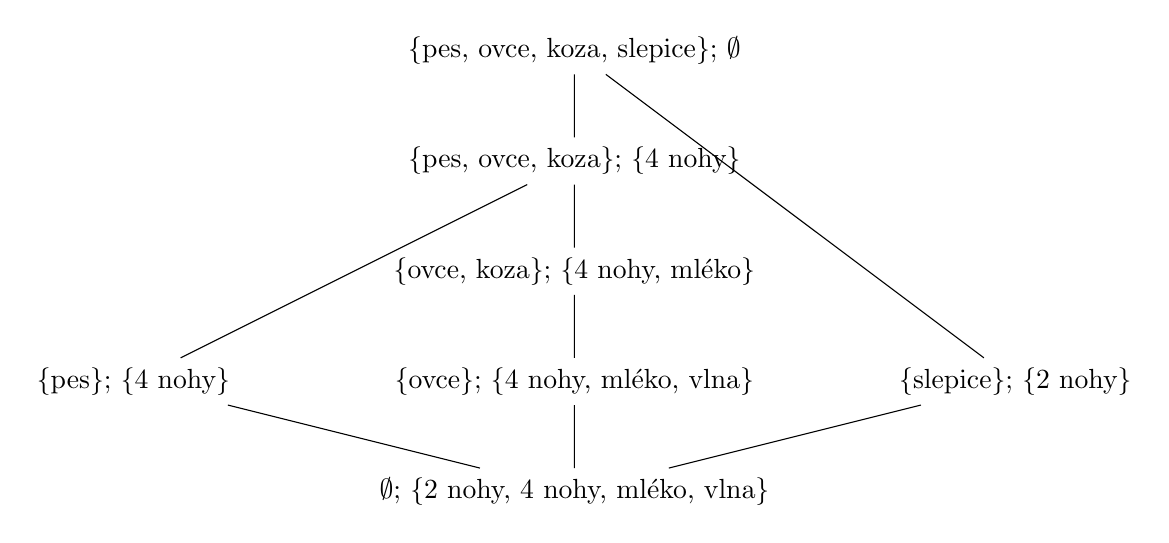
\begin{tikzpicture}[scale=.7]
\node (e6) at (0,-4) {$\emptyset$; \{2 nohy, 4 nohy, mléko, vlna\}};
\node (e5) at (-8,-2) {\{pes\}; \{4 nohy\}};
\node (e4) at (0,-2) {\{ovce\}; \{4 nohy, mléko, vlna\}};
\node (e1) at (8,-2) {\{slepice\}; \{2 nohy\}};
\node (e3) at (0,0) {\{ovce, koza\}; \{4 nohy, mléko\}};
\node (e2) at (0,2) {\{pes, ovce, koza\}; \{4 nohy\}};
\node (e7) at (0,4) {\{pes, ovce, koza, slepice\}; $\emptyset$};
\draw (e6) -- (e5) -- (e2) -- (e7) -- (e1) -- (e6) -- (e4) -- (e3) -- (e2);
\end{tikzpicture}
\end{center}

\subsection{Svazy (pro doplnění, asi není nutné úplně znák k FCA)}
Svaz je algebra $(L, \cap, \cup)$ s dvěma základními binárními operacemi $x\cap{}y$ \textbf{spojení (suprémum)} (sup(x, y)) a $x\cup{}y$ \textbf{průsek (infimum)} (inf(x, y)), které mají následující vlastnosti:
\begin{enumerate}
\item \textbf{Univerzalita (jednoznačnost)} -- $\forall x,y \,\exists z \,\,\, x \cap y = z\quad|\quad\forall x,y \exists\, z \,\,\, x \cup y = z$.
\item \textbf{Asociativita} -- $x \cap (y \cap z) = (x \cap y) \cap z \quad|\quad x \cup (y \cup z) = (x \cup y) \cup z$.
\item \textbf{Komutativita} -- $x \cap y = y \cap x \quad|\quad x \cup y = y \cup x$.
\item \textbf{Absorbce} -- $x \cap (x \cup y) = x \quad|\quad x \cup (x \cap y) = x $.
\end{enumerate}

\subsubsection{Typy svazů}
\begin{enumerate}
\item \textbf{Distributivní} -- platí zde axiomy distributivity a neobsahuje ani \textbf{diamant} ani \textbf{pentagon}: $x \cup (y \cap z) = (x \cup y) \cap (x \cup z) \quad|\quad x \cap (y \cup z) = (x \cap y) \cup (x \cap z) $.

\begin{figure}[H]
	\centering
	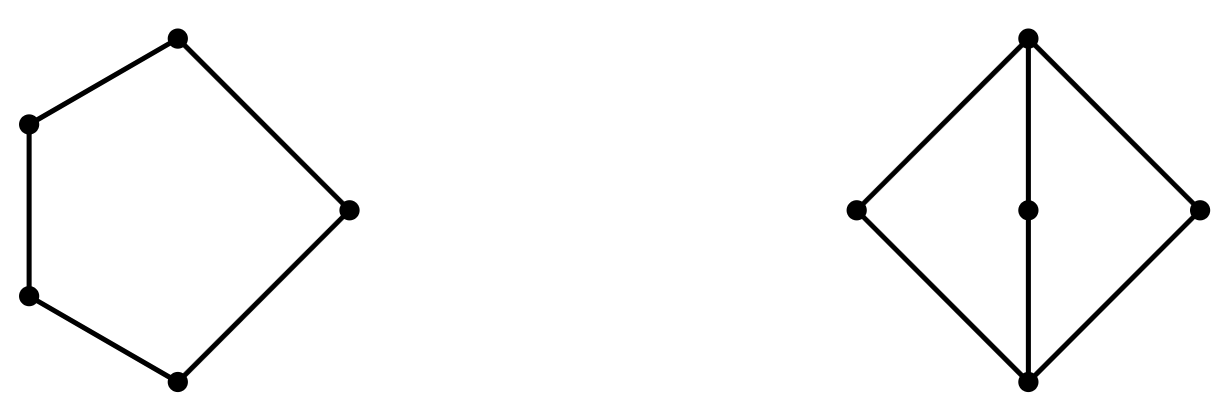
\includegraphics[width=.4\textwidth]{assets/pentagon_diamant}
\end{figure}
\item \textbf{Modulární} -- slabší reprezentace distributivity, \textbf{nesmí} obsahovat \textbf{pentagon}, $a \geq c: a \land (b \lor c) = (a \land b) \lor c$.
\item \textbf{Komplementární} -- platí zde, že pro každý prvek $ x $ existuje komplement $x' $, kdy: $x \cap x' = $ [svazová 0] a $x \cup x' = $ [svazová 1]
\item \textbf{Booleovský svaz} -- komplementární $\land$ distributivní
\end{enumerate}

\subsubsection{Vlastnosti svazů}
Pro každé dva prvky v množině existuje \textbf{sup} a \textbf{inf}. \textbf{Úplný svaz} -- nastane tehdy, zda pro \textbf{libovolné neprázdné podmnožiny existuje} sup a inf. U svazů můžeme dále získat tyto vlastnosti:
\begin{itemize}
\item \textbf{Minimum a maximum} -- žádný není menší/větší než $a$ (vrchol diagramu).
\item \textbf{Nejmenší a největší} -- \textbf{pouze jeden} nejmenší/největší prvek, pokud je jich více, \textbf{neexistuje} největší/nejmenší prvek.
\item \textbf{Dolní (L(A)) a horní (U(A)) závora} -- všechny prvky jsou $\leq/\geq$ než A,
\item \textbf{Infimum} -- nejmenší prvek dolní závory.
\item \textbf{Supremum} -- nejmenší prvek horní závory.
\end{itemize}

\subsection{Asociační pravidla}
Termín asociační pravidla široce zpopularizoval počátkem 90. let v souvislosti s analýzou nákupního košíku. Při této analýze se zjišťuje, jaké druhy zboží si současně kupují zákazníci v supermarketech (např. pivo a párek). \textbf{Jde} tedy \textbf{o hledání vzájemných vazeb} (\textbf{asociací}) \textbf{mezi různými položkami} sortimentu prodejny. Přitom není upřednostňován žádný speciální druh zboží jako závěr pravidla.

\subsubsection{Základní charakteristika pravidel}
U pravidel vytvořených z dat nás obvykle zajímá kolik příkladů splňuje \textbf{předpoklad} a kolik \textbf{závěr} pravidla, kolik příkladů splňuje předpoklad i závěr \textbf{současně}, kolik příkladů splňuje předpoklad a \textbf{nesplňuje} závěr…. Tedy, zajímá nás, jak pro pravidlo:
\begin{equation}
Ant \Rightarrow Suc, \quad\textrm{ kde } Ant, Suc \subseteq I \textrm{ (položky)}
\end{equation}
kde $ Ant $ (\textbf{předpoklad}, levá strana pravidla, \textbf{antecedent}) a $ Suc $ (\textbf{závěr}, pravá strana pravidla, \textbf{sukcedent}) jsou kombinace kategorií, pro něž příslušná \textbf{kontingenční tabulka} vypadá následovně:
\begin{table}[H]
	\centering
	\begin{tabular}{l|ll}
		&  $ Suc $ & $ \neg Suc $ \\\hhline
	$ Ant $	&a  & b \\
	$ \neg Ant $	& c & d
	\end{tabular}
\end{table}
\begin{itemize}
\item $Ant \land Suc$ -- \textbf{a} je počet objektů {pokrytých současně předpokladem i závěrem},
\item $Ant \land \neg Suc)$ -- \textbf{b} je počet objektů {pokrytých předpokladem a nepokrytých závěrem},
\item $\neg Ant \land Suc)$ -- \textbf{c} je počet příkladů {nepokrytých předpokladem ale pokrytých závěrem},
\item $\neg Ant \land \neg Suc)$ -- \textbf{d} je počet příkladů {nepokrytých ani předpokladem ani závěrem}. 
\end{itemize}

\subsubsection{Základní charakteristiky asociačních pravidel}
\begin{itemize}
\item \textbf{Support (podpora)} -- relativní četnost objektů splňující předpoklad i závěr, jinými slovy {\scriptsize$\frac{\textrm{počet splňující výstup}}{\textrm{počet položek}}$}:
\begin{equation}
sup(Ant \Rightarrow Suc) = \frac{a}{a + b + c + d}, \, \in \, \langle 0; 1 \rangle.
\end{equation}
\item \textbf{Confidence (spolehlivost)} -- podmíněná pravděpodobnost závěru pokud platí předpoklad, tedy {\scriptsize$\frac{\textrm{podpora obou}}{\textrm{podpora závěru}}$}:
\begin{equation}
conf(Ant \Rightarrow Suc) = \frac{sup(Ant \cup Suc)}{sup(Suc)} = \frac{a}{a + b}.
\end{equation}
\item Další: \textbf{pokrytí}, \textbf{zajímavost}, \textbf{závislost}.
\end{itemize}

\subsection{Hledání často se opakujících množin položek)}
Frequent item set je množina, kde $sup(K) \geq \gamma$, máme tedy stanovenou \textbf{minimální podporu}. Pokud je např. $\gamma = 0,3$ pak je minimální podpora 30\%.

\subsubsection{Generování kombinací}
Základem všech algoritmů pro hledání asociačních pravidel je \textbf{generování kombinací (konjunkcí) hodnot atributů}. Při generování vlastně procházíme (prohledáváme) prostor všech přípustných konjunkcí. Metod je několik:
\begin{itemize}
\item do \textbf{hloubky},
\item do \textbf{šířky},
\item \textbf{heuristicky},
\end{itemize}

\subsubsection{Algoritmus apriori}
Jedná se o nejznámějším algoritmus pro hledání asociačních pravidel Jádrem algoritmu je \textbf{hledání často se opakujících množin} položek (frequent itemsets). Jedná se kombinace (konjunkce) kategorií, které dosahují předem zadané četnosti (\textbf{minimální podpory}) v datech.

\begin{figure}[H]
	\centering
	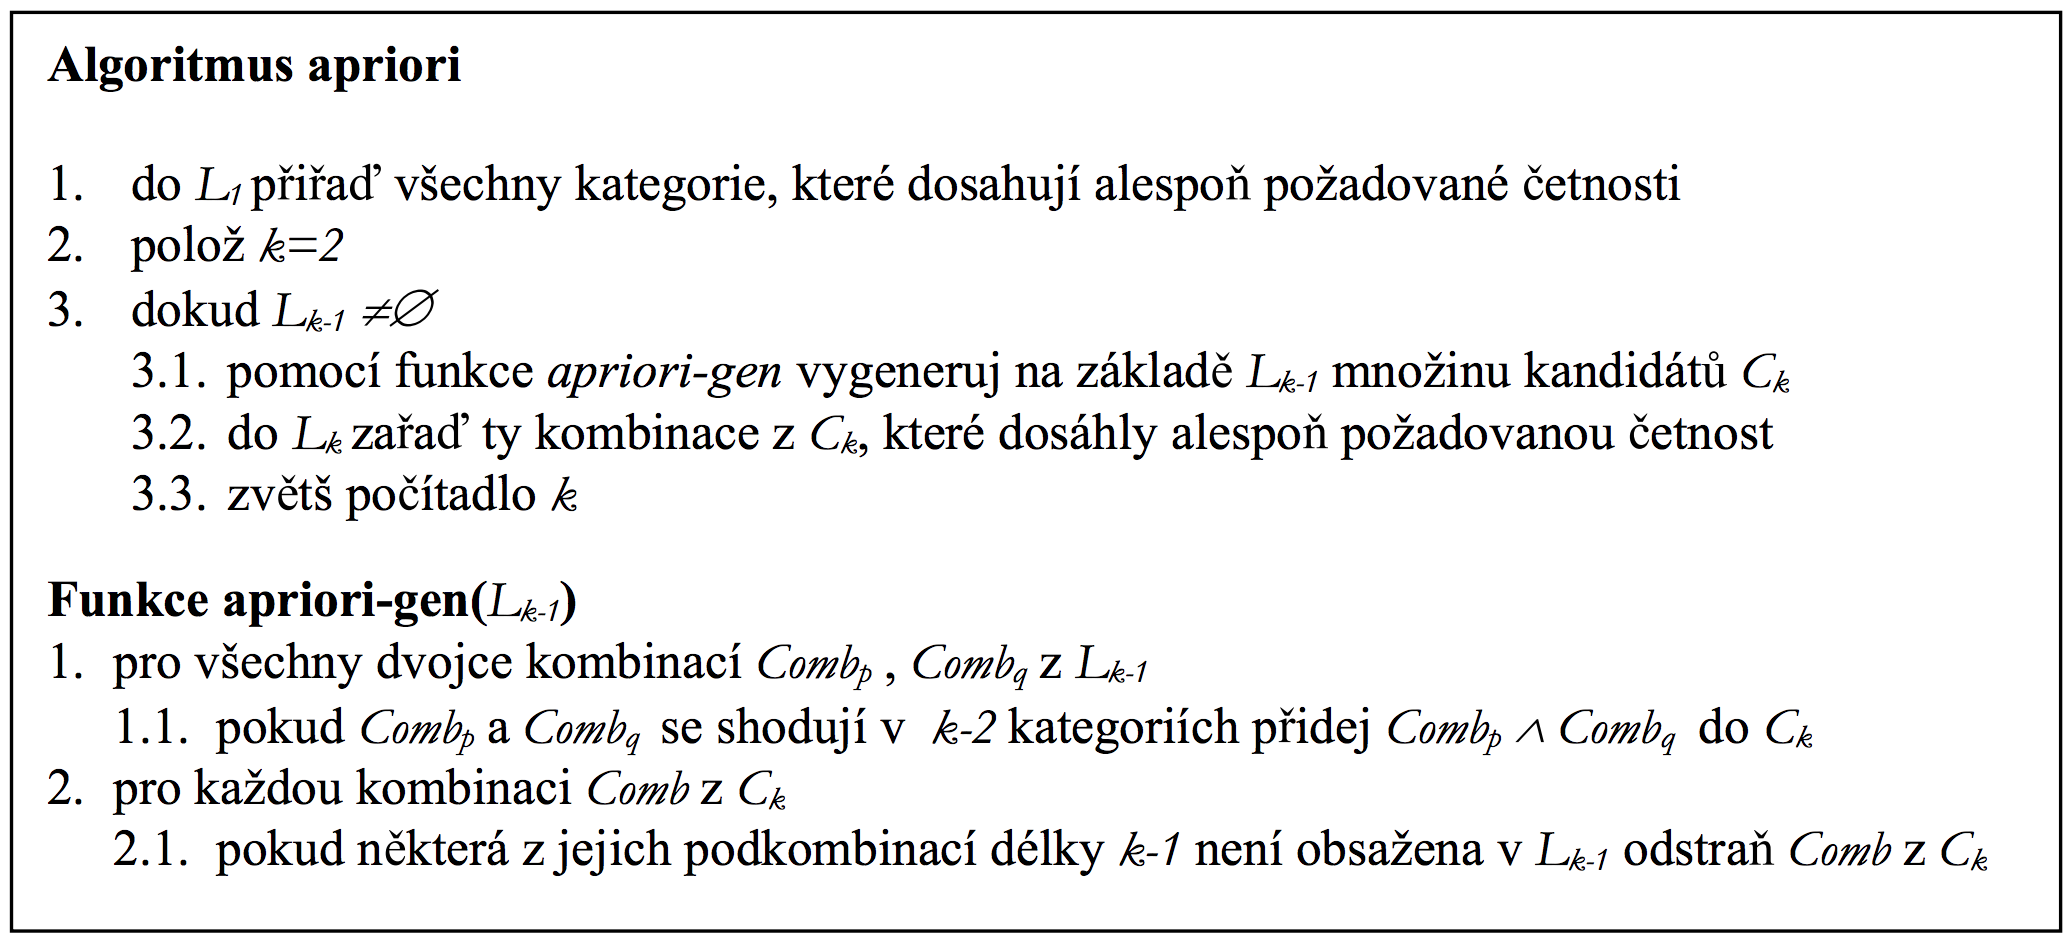
\includegraphics[width=\textwidth]{assets/apriori.png}
\end{figure}

Při hledání kombinací délky $ k $, které mají vysokou četnost se využívá toho, že \textbf{již známe kombinace délky} $ k-1 $. Při vytváření kombinace délky $ k $ spojujeme kombinace délky $ k-1 $.

Jde tedy o \textbf{generování kombinací ,,do šířky''}. Přitom pro vytvoření jedné kombinace délky $ k $ požadujeme, aby všechny její podkombinace délky $ k-1 $ \textbf{splňovaly požadavek na četnosti}. Tedy např. ze tříčlenných kombinací $\{A_1A_2A_3,  \,A_1A_2A_4, \, A_1A_3A_4, \,A_1A_3A_5,  \,A_2A_3A_4\}$ dosahujících požadované četnosti vytvoříme \textbf{pouze jedinou čtyřčlennou} kombinaci $ A_1A_2A_3A_4 $. Kombinaci $ A_1A_3A_4A_5 $ sice lze vytvořit spojením $ A_1A_3A_4 $ a
$ A_1A_3A_5 $, ale mezi tříčlennými kombinacemi chybí $ A_1A_4A_5 $ i $ A_3A_4A_5 $.

\subsubsection{Algoritmus Next Closure}
Slouží k vytváření formálních kontextů, \textbf{vyhledáváním nejmenších intentů}, postup:
\begin{enumerate}
\item Začnu s následující tabulkou:
\begin{table}[H]
	\centering
	\begin{tabular}{l|l|l|l|l|p{6cm}}
		\multirow{2}{*}{$ A $} & \multirow{2}{*}{$ i $} & \multirow{2}{*}{$ A \cap \{1 \ldots i - 1\} \cup \{i\} = B' $ } & \multirow{2}{*}{$ cl(B') = B $ } & \multirow{2}{*}{$B \setminus A $  } & je-li $B \setminus A = \{i\}$ nebo větší $\rightarrow$ ANO  \\
		&                   &                   &                   &                   & je-li $B \setminus A = \{j\}$, kde $j < i$ $\rightarrow$ NE \\\hhline
		$\emptyset$ & 5  &  &  &  & 
	\end{tabular}
\end{table}
\item Do $A$ vložím prázdnou množinu a $i$ nastavím na nejvyšší intent (pořadí).
\item Udělám průnik s $A \cap \{1 \ldots i - 1\} \cup \{i\} = B'$ $\rightarrow$ průnik Ačka s intenty od $ 1 $ do $ i-1 $, k tomu přidám $i$. Př.: $A = \{1, 3, 4\}, i = \{3\} \Rightarrow B' = \{1, 3\}$.
\item Udělám closure ($B'$) $\rightarrow$ intent na extent $\rightarrow$ extent na intent $\Rightarrow B'^{\downarrow \uparrow}$.
\item Od $B$ odečtu $A$.
\item Je-li:
\begin{itemize}
\item $B \setminus A = \{i\}$ a větší tak ANO [je-li nejmenší prvek z $B \setminus A$ roven nebo větší než $\{i\}$],
\item $B \setminus A = \{j\}$ kde $j < i$ tak NE [je-li nejmenší prvek z $B \setminus A$ menší než i pak NE].
\end{itemize}
\item Pokud:
\begin{itemize}
\item ANO $\rightarrow$ do $A$ dosadíme $cl(B') = B$ a $i$ nastavíme na nejvyšší intent,
\item NE $\rightarrow$ do $A$ neměním a snížíme $i$ o $-1$.
\end{itemize}
\item Skončím když je $A$ rovno celé množině extentů.
\end{enumerate}

\paragraph{DÚLEŽITÉ} V $i$ přeskakuju hodnoty, které jsou v $A$ [výjde pro ně $\emptyset \rightarrow$ neřeším].

\subsubsection*{Příklad}
\begin{table}[H]
	\centering
	\begin{tabular}{l|lllll}
		 &  $y_1$& $y_2$ & $y_3$& $y_4$& $y_5$ \\\hhline
		$x_1$ &  0& 1 & 0 &  1& 1 \\
		$x_2$& 0 & 1 & 1 & 0 & 0 \\
		$x_3$& 1 & 1 &  0& 1 & 1 \\
		$x_4$& 1 & 1 & 1 & 0 & 0 \\
		$x_5$& 1 & 0 & 1 & 1 & 0 \\
		$x_6$& 1 & 0 & 0 &  1& 0
	\end{tabular}
\end{table}


\begin{tabular}{l|l|l|l|l|p{3cm}}
\multirow{2}{*}{$ A $} & \multirow{2}{*}{$ i $} & \multirow{2}{*}{$ A \cap \{1 \ldots i - 1\} \cup \{i\} = B' $ } & \multirow{2}{*}{$ cl(B') = B $ } & \multirow{2}{*}{$B \setminus A $  } & \multirow{2}{*}{ANO / NE }  \\
&&&&&\\ \hhline
$\emptyset$ & 5  & 5 &  2, 4, 5&  2, 4, 5&  N [2 < 5] \\
$\emptyset$ & 4  & 4 &  4&  4&  A [4 $\geq$ 4] $\leftarrow$ $i_n$ \\
4 & 5  & 4, 5 &  2, 4, 5&  2, 5&  N [2 < 5] \\
4 & 3 [skip $i$]  & 3 &  3&  3&  A [3$\geq$ 3] $\leftarrow$ $i_{n - 1}$ \\
3 & 5  & 3, 5 &  1, 2, 3, 4, 5&  1, 2, 4, 5&  N [1 < 5] \\
&&\vdots&&& \\
1, 2, 3, 4, 5&&KONEC&&&A $i_{1}$
\end{tabular}